\documentclass[../main.tex]{subfiles}
\begin{document}

\section{Билет 2. Постановка задачи Коши для уравнения 2-го порядка с частными производными в \texorpdfstring{$\R^n$}{R\textasciicircum n} с линейной старшей частью. Понятие о корректности задачи Коши. Пример Адамара некорректности задачи Коши для уравнения Лапласа.}
% Затехал: Рязанов Андрей
В области $\Omega \subset \R^n$ задано уравнение:
\begin{equation}
\label{eq::2::init}
\sum\limits_{i,j=1}^{n} a_{ij}(x)\frac{\subd^2u}{\subd x_i\subd x_j} + F(x, u, \nabla u) = 0
\end{equation}
и поверхность $S:\ \omega(x) = \omega(x_1, \dots, x_n) = 0,\ \omega \in C^2(\Omega)$ и $\mathrm{grad}(\omega) \not= 0$ на $\Omega$ (нет особых точек).\\
На поверхности задано гладкое некасательное поле $\vec{\nu} = (\nu_1(x), \dots, \nu_n(x)),\ \; \langle \vec{\nu}, \vec{n} \rangle \not= 0$.
\begin{definition}[Задача Коши]
В $U(x^0)\subset\Omega,\ x^0 \in S$, найти то решение уравнения \eqref{eq::2::init}, которое удовлетворяет двум условиям:
\begin{enumerate}
\item $u(x)|_{S\cap U(x^0)}=u_0(x)$
\item $\left.\dfrac{\subd u}{\subd \vec{\nu}}\right|_{S\cap U(x^0)} = u_1(x)$ -- выводящая производная

Здесь введена производная по направлению: $\dfrac{\subd u}{\subd \vec{\nu}} = \brs{\vec{\nu}, \nabla u} = \displaystyle\sum\limits_{k=1}^{n} \nu_k(x)\dfrac{\subd u}{\subd x_k}(x) $
\end{enumerate}
\end{definition}
Может не быть непрерывной зависимости от начальных данных.\\
Функции $u_0, u_1$ произвольно брать, вообще говоря, нельзя.


Далее определим характеристическую поверхность.\\
Пусть $S$ -- гиперплоскость $x_n = 0$. Нормаль $\vec{n} = (0,0,\dots,0, 1)^T,\\
u(x_1, \dots, x_{n-1}, 0) = u_0(x_1, \dots, x_{n-1}),\quad \dfrac{\subd u}{\subd\vec{n}} = \dfrac{\subd u}{\subd x_n} = u_1(x_1, \dots, x_{n-1}) $

Мы знаем значения функции на гиперплоскости.\\
Знаем градиент:
\begin{equation*}
\left\{\begin{aligned}
\frac{\subd u}{\subd x_1}(x_1, \dots, x_{n-1}, 0) &= \frac{\subd u_0}{\subd x_1}(x_1, \dots, x_{n-1})\\ 
&\vdots \\
\frac{\subd u}{\subd x_{n-1}}(x_1, \dots, x_{n-1}, 0) &= \frac{\subd u_0}{\subd x_{n-1}}(x_1, \dots, x_{n-1})
\end{aligned} \right\}
+\left\{\frac{\subd u}{\subd x_n}(x_1,\dots,x_{n-1},0)\right\} = u_1
\end{equation*}
Мы знаем и вторые производные: берём указанные сверху производные и дифференцируем вдоль поверхности, получим \[\frac{\subd^2u}{\subd x_i\subd x_j}(x_1,\dots,x_{n-1}, 0) = \frac{\subd^2u_0}{\subd x_i\subd x_j},\ 1\le i,j \le n-1 \]
\[\frac{\subd^2u}{\subd x_n\subd x_i}(x_1,\dots,x_{n-1}, 0) = \frac{\subd u_1}{\subd x_i}(x_1,\dots,x_{n-1}),\ 1\le i\le n-1\]

Не нашли только $\displaystyle\spd{u}{x_n}{x_n}$. До этого мы вообще еще не использовали уравнение:

$$\displaystyle\sum\limits_{i,j=1}^{n-1}a_{ij}u_{x_ix_j} + \displaystyle\sum\limits_{j=1}^{n-1}\left[a_{nj}u_{x_nx_j} + a_{jn}u_{x_jx_n}\right] + \underbrace{a_{nn}u_{x_nx_n}}_{\substack{\text{только это слагаемое}\\ \text{еще не определено}}} + F(x, u, \nabla u) = 0 $$
Если $a_{nn}(x) = 0$ на нашей гиперплоскости, то эту гиперплоскость назовём {\bf характеристической}. На характеристической гиперплоскости полученное уравнение задаёт функциональную связь $u_0$ и $u_1$ -- эта связь называется {\bf условием совместности}.

Теперь переходим к произвольной поверхности: заменим координаты так, чтобы локально поверхность была гиперплоскостью:
\[y = y(x) = \begin{cases} y_1 = y_1(x_1,\dots, x_n) \\ \vdots \\ y_{n-1} = y_{n-1}(x_1,\dots,x_n) \\ y_n = \omega(x_1,\dots,x_n) \end{cases} \]
$\To$ после преобразования $\omega=0 \Equiv y_n=0$.\\
Найдём это преобразование: возьмем $\vec{n} = \nabla \omega$.
\begin{center}
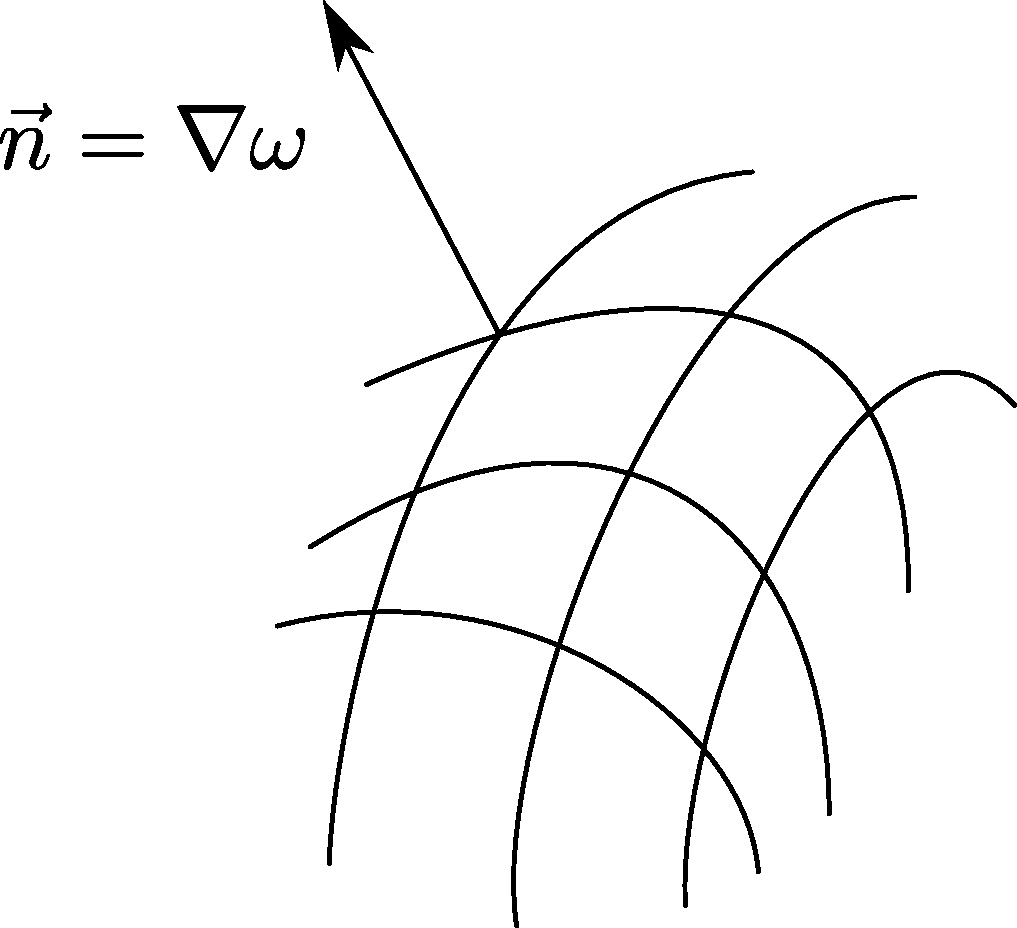
\includegraphics[width=0.22\textwidth]{./pic 2_1.pdf}
\end{center}
Дополним $\vec{n}$ до базиса -- получим $\rbrs{\vec{l}_1,\dots,\vec{l}_{n-1},\vec{n}}$. Ортогонализуем -- получим $\rbrs{\vec{e}_1,\dots,\vec{e}_{n-1},\vec{n}}.$ Возьмем такое преобразование:
\[ \vec{y}(\vec{x}) = \begin{cases} y_1 = \brs{\vec{x}-\vec{x}_0} \cdot \vec{e}_1 \\ \vdots \\ y_{n-1} = \brs{\vec{x}-\vec{x}_0} \cdot \vec{e}_{n-1} \\ y_n = \omega(\vec{x}) \end{cases}\]
Проверим $|J(x^0)|\not=0: \quad |J(x^0)| = 
\begin{vmatrix} 
\displaystyle\pd{y_1}{x_1}(x^0) & \cdots & \displaystyle\pd{y_1}{x_n}(x^0) \\
\cdots &\cdots &\cdots \\
\displaystyle\pd{\omega}{x_1}(x^0) & \cdots & \displaystyle\pd{\omega}{x_n}(x^0) \\
\end{vmatrix} $. Строки матрицы -- компоненты ОНБ $\To |J|\not= 0.$\\
Значит, это диффеоморфизм класса $C^2$.\\
В новых переменных: $\displaystyle\sum\limits_{k,l=1}^{n}\hat{a}_{kl}(y)\displaystyle\spd{\hat{u}}{y_k}{y_l} + \hat{F}(y, \hat{u}, \nabla_y \hat{u}) = 0 $.\\
Условие характеристичности поверхности: $\hat{a}_{nn} = \displaystyle\sum\limits_{i,j=1}^{n} a_{ij}[x(y)]\displaystyle\pd{y_n}{x_i}\displaystyle\pd{y_n}{x_j} = 0$.

\begin{definition}[Характеристическая поверхность]
Гладкая поверхность $S$ называется {\bf характеристикой}, если в точках этой поверхности выполнено равенство  $\displaystyle\sum\limits_{i,j=1}^{n}a_{ij}\omega_{x_i}\omega_{x_{j}} = 0$.
\end{definition}

\begin{example}
$\displaystyle\pdd{u}{x} - \displaystyle\pdd{u}{y} = 0.\quad S$ -- прямая $x=y, \quad \vec{n} = \left(-\dfrac1{\sqrt{2}}, \dfrac1{\sqrt{2}}\right);\quad \displaystyle\pd{u}{\vec{n}} = -\dfrac{u_x}{\sqrt2} + \dfrac{u_y}{\sqrt2} = u_1$

Производная $\displaystyle\d{u_1}{\vec l} = \left(\vec{l}, \nabla\displaystyle\pd{u}{\vec{n}}\right) = \dfrac1{\sqrt{2}}\displaystyle\pd{}{x}\left[-\dfrac1{\sqrt2}u_x + \dfrac1{\sqrt{2}}u_y\right] + \dfrac1{\sqrt{2}}\displaystyle\pd{}{y}\left[-\dfrac1{\sqrt2}u_x + \dfrac1{\sqrt{2}}u_y\right] = 0.$

Значит, любую функцию на $S$ задать нельзя; прямая $x=y$ -- характеристика.
\end{example}
\vspace{5pt}


\begin{example}
$u_{tt}-a^2\Delta_xu = f(t,x),\ x\in\R^3\ $(волновое уравнение).

Характеристическое уравнение: $\brs{\displaystyle\pd{\omega}{t}}^2 - a^2(\mathrm{grad}(\omega))^2 = 0$

Этому уравнению удовлетворяет $\omega(t,x) = \underbrace{a^2t^2 - \vec{x}^2 = 0}_{\text{конус}}$.
\end{example}



\begin{example}
$u_{t}-a^2\Delta_xu = f(t,x)\ $(уравнение теплопроводности).

Характеристическое уравнение: $-a^2[\omega_{x_1}^2 + \dots + \omega_{x_n}^2] = 0\ \To \ \omega_{x_i} = 0\ \forall i=\overline{1,n}$

Так как $\nabla \omega \not= 0 $, мы требуем $\omega_t \not=0$. 

Подходит $\omega(t,x) = t-C = 0 \qquad   \Rightarrow \qquad \underline{\text{гиперплоскости}\ t=C}$.
\end{example}



\begin{example}
$\Delta u(x) = f(x)\ \text{(ур-е Пуассона)},\ x\in\R^n;$

Характеристическое уравнение: $\; a^2[\omega_{x_1}^2+\dots+\omega_{x_n}^2] = 0 \ \To\ \omega_{x_i} = 0\ \forall i=\overline{1,n}.$

А мы требовали $\nabla \omega \not=0\ \To\ $ у уравнения эллиптического типа нет характеристик.
\end{example}

\begin{offtop}
Пусть $S:\ \omega(\vec{x}) = 0,\ \omega(\vec{x}) \in C^2(\Omega),\ \nabla\omega\not=0\ \forall \vec{x}\in \Omega$ (гладкая поверхность, нормаль меняется непрерывно).\\
Будем называть точку $\vec{x}_0 \in S\ \text{{\bf характеристической}, если }\ \displaystyle\sum\limits_{i,j=1}^{n}a_{ij}(\vec{x}_0)\omega_{x_i}(\vec{x}_0)\omega_{x_j}(\vec{x}_0) = 0.$
\end{offtop}
\begin{center}
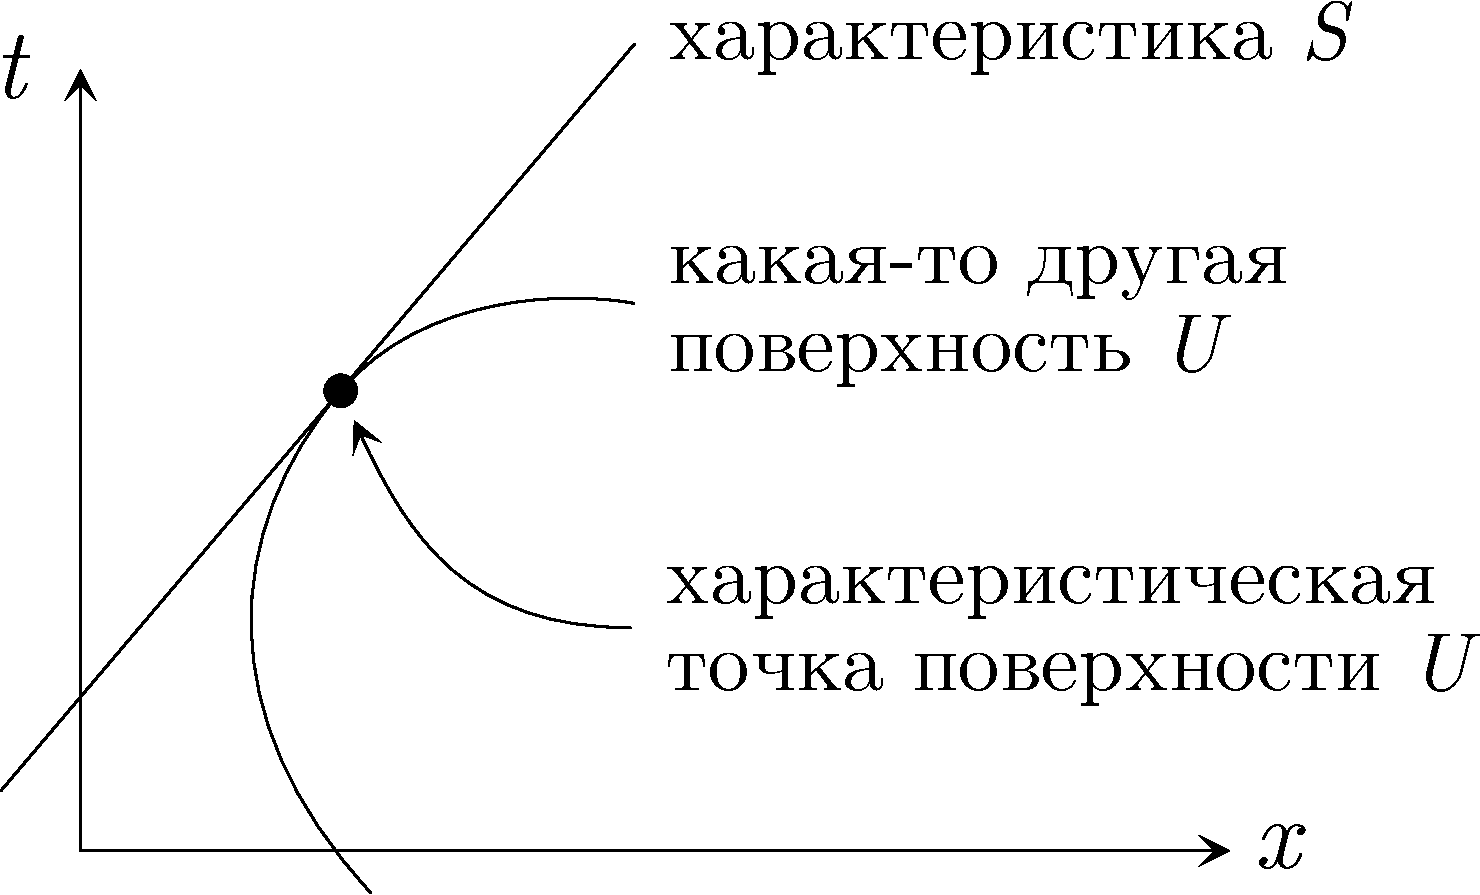
\includegraphics[width=0.3\textwidth]{pic 2_2.pdf}
\end{center}

\medskip

Функция $u(\vec{x}) = u(x_1,\dots,x_n)$ называется {\bf вещественно-аналитической} в $\vec{x}_0$, если в некоторой $U_{\varepsilon}(\vec{x}_0)$ она представима в виде $u(\vec{x}) = \displaystyle\sum\limits_{|\alpha|>0}u_{\alpha}(\vec{x}-\vec{x}_0)^{\alpha},$ где $\alpha$ -- мультииндекс, $u_{\alpha} \in \R, \qquad (\vec{x}-\vec{x}_0)^{\alpha} = (x_1-x_1^0)^{\alpha_1}\cdot\dots\cdot(x-x_n^0)^{\alpha_n}$

\begin{theorem}[Ковалевской]
Пусть в уравнении $\displaystyle\sum\limits_{i,j=1}^{n} a_{ij}(\vec{x})\frac{\subd^2u}{\subd x_i\subd x_j} + F(\vec{x}, u, \nabla u) = 0$:
\begin{itemize}[noitemsep]
\item все $a_{ij}(\vec{x})$ вещественно-аналитические в $\vec{x}_0$ 
\item $F(\vec{x}, u, \nabla u)$ --вещественное-аналитическая в $(\vec{x}_0, u_0(\vec{x}_0), \nabla u(\vec{x}_0))$ соответственно 
\item $\omega(\vec{x})$ вещественно-аналитическая в $\vec{x}_0$
\item $\vec{x}_0$ -- не характеристическая точка $S$
\item $u_0,\ u_1$ -- вещественно-аналитические в $\vec{x}_0$.
\end{itemize}
Тогда: 
\begin{itemize}[noitemsep]
\item $\exists U_{\varepsilon}(\vec{x}_0)$ : в ней $\exists$ вещественно-аналитическое решение Задачи Коши (ЗК)
\item оно единственно в классе вещественно-аналитических функций.
\end{itemize}
\end{theorem}

\subsection*{Понятие о корректности}

Рассмотрим абстрактную дифференциальную задачу:

\begin{equation}
\label{eq::2::diff}
\tag{*}
\begin{cases} L(\vec{x}, D)u(\vec{x}) = f(\vec{x}),\ \vec{x} \in \Omega \subseteq \R^n  \\
B_j(\vec{x},D) u(\vec{x}) = g_j(\vec{x}),\ \vec{x}\in \Gamma,\ j\in\overline{1,m},
\end{cases}
\end{equation}
$L$ -- линейный дифференциальный оператор порядка $p$\\
$B_j$ -- конечное семейство линейных дифференциальных операторов в $\Gamma \subset \bar{\Omega}$.

\begin{center}
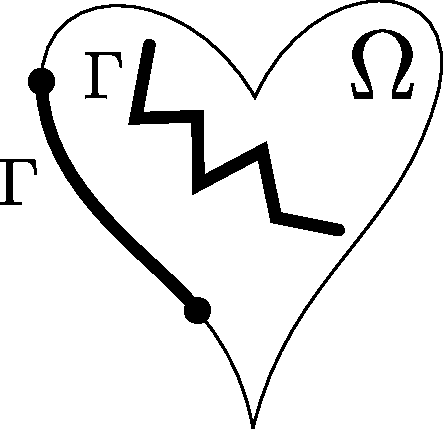
\includegraphics[width=0.1\textwidth]{pic 2_3.pdf}
\end{center}

\begin{definition}
Пусть $F(\Omega)$ и $U(\Omega)$ -- линейные нормированные пространства функций (ЛНП) на $\Omega$, \; $G_1(\Gamma),\dots G_m(\Gamma)$ -- ЛНП на $\Gamma$.

Тогда если $\forall f(\vec{x}) \in F(\Omega),\; \forall g_j(\vec{x}) \in G_j(\Gamma)$ решение краевой задачи \eqref{eq::2::diff} существует, единственно в $U(\Omega)$ и для него справедлива оценка
\begin{equation}
    \norm{u}_{U(\Omega)} \leq C\norm{f}_{F(\Omega)} + \sum\limits_{j=1}^{m}c_j\norm{g_j}_{G_j(\Gamma)}
\label{eq::2::neq}
\tag{**}
\end{equation}
то {\bf задача корректна по отношению к выбранному набору пространств.}
\end{definition}

\begin{example}[Адамара]
Рассмотрим задачу Коши для уравнения Лапласа:

$\begin{cases} u_{xx}+u_{yy} = 0 \\
u|_{y=0} = u_0(x) = e^{-\sqrt{n}}\cos{nx} \rightrightarrows 0\ \text{вместе со своими производными} \\
u_y|_{y=0} = u_1(x) \equiv 0
\end{cases}$

При $u_0 = 0 \hookrightarrow u\equiv 0$. Если задача корректна, то при увеличении $n$ решения должны $\rightarrow 0$. 

Функции $u_n=e^{-\sqrt{n}}\cos{nx}\ch{ny}$ -- решения.

Но $u_n(0, y^*) = e^{-\sqrt{n}}\ch{ny^*} > \frac1{2}e^{-\sqrt{n}}e^{ny^*} \rightarrow \infty$

Неравенство \eqref{eq::2::neq} не выполнено.
\end{example}
\end{document}